\documentclass[a4paper,12pt]{article}
\usepackage[mag=1000,tikz]{newlistok}

\ВключитьКолонтитул

\УвеличитьШирину{1.4cm}
\УвеличитьВысоту{2.3cm}

\Заголовок{Комплексные числа и движения}
\НомерЛистка{41}
% \renewcommand{\spacer}{\vspace{0.9pt}}
\ДатаЛистка{2.12 -- 11.12.2019}
% 45 задач
\Оценки{30/25/20}


\begin{document}

\СоздатьЗаголовок


\пзадача
Докажите, что если $zw=0$, то либо $z=0$, либо $w=0$.
\кзадача

\пзадача
Докажите, что если и сумма, и произведение двух комплексных чисел вещественны, то либо оба этих числа вещественны, либо сопряжены.
\кзадача






\пзадача
Решите уравнения:\\
\вСтрочку
\пункт
$z^2=e^{\frac{i \pi}{3}}$;
\пункт
$z^2=5-12i$;
\пункт
$z^2+(2i-7)z+13-i=0$;
\пункт
$\ol z=z^2$;
\пункт
$\ol z=z^3$;
$z^3+z^2+z+1=0$.
\кзадача


% \задача
% Нарисуйте множество комплексных чисел, для которых:\\
% \вСтрочку
% \пункт $|z-1|=2|z-i|$;
% \пункт $z^2+\ol z^2=4$;
% \пункт $|z-1|-|z+1|\leq3$;
% \пункт $|z-1|+|z+1|=3$;
% \пункт $z+\ol z=2|z-1|$.
% \кзадача

% \задача
% При каких вещественных $c$ все комплексные корни уравнения $z^3 + z^2 = c$ по модулю не превосходят единицу?
% \кзадача

\задача
Пусть $z$ и $w$ --- ненулевые различные комплексные числа. Верно ли, что точки $z$, $w$, $\frac1{\overline{z}}$, $\frac1{\overline{w}}$ лежат на одной окружности?
\кзадача


% \задача
% Нарисуйте: % множество комплексных чисел $z$, для которых\\
% \вСтрочку
% \!\!\!\! \пункт \!\!\!\! $\{ z\in\Cbb\,\,|\,\,z^n+1=0\}$;
% \пункт $\{z\in\Cbb\,\,|\,\,2\geq|z-i|\}$;
% \пункт $\{z\in\Cbb\,\,|\,\,{\rm Re}\left(\frac{1}{z}\right)=1\}$;
% \пункт $\{\frac{1+ti}{1-ti}\,\,|\,\,t\in\R\}$.
% \кзадача



\задача
Даны два комплексных числа $a$ и $b$. Опишите множество таких $z\in\Cbb$,
что $(z-a)/(z-b)$ —
\невСтрочку
\пункт
вещественное число;
\пункт
чисто мнимое число.
\пункт
Каков геометрический смысл аргумента этого числа?
\пункт
Докажите, что треугольники $\triangle z_1z_2z_3$ и $\triangle w_1w_2w_3$ подобны тогда и только тогда,
когда простые отношения точек $z_1, z_2, z_3$ и $w_1, w_2, w_3$ равны или сопряжены.
% \пункт Какое множество точек задается уравнением $(z-a)(\bar z - \bar b)=(z-b)(\bar z - \bar a)$?
\кзадача

\задача
Опишите геометрически преобразование плоскости, заданное формулой:
\невСтрочку
% \таа
{\пункт $z\longmapsto z+w$, где $w$ --- комплексное число;}
{\пункт $z\longmapsto kz$, где $k$ --- вещественное число;}
% \таа
{\пункт $z\longmapsto 2z+1$;}
{\пункт $z\longmapsto \bar z$;}
% \таа
{\пункт $z\longmapsto e^{i \alpha }z$, где $0 \leq \alpha < 2\pi$;}
{\пункт $z\longmapsto wz$, где $w$ --- произвольно.}
\кзадача


\задача
Запишите %в виде
как функцию комплексной переменной (можно использовать переменную $z$, комплексные числа и операции сложения, вычитания, умножения, деления, сопряжения)
\невСтрочку
% \таа
{\пункт симме\-трию относительно оси $y$;}
{\пункт ортогона\-ль\-ную проекцию на ось $x$;}
% \таа
{\пункт центральную симметрию с центром $A$;}
{\пункт поворот на угол $\varphi$ относительно~точки~$A$;}
% \таа
{\пункт гомотетию с коэффициентом $k$ и центром $A$;}
{}
\пункт скользящую симметрию относительно прямой $y=3$ со сдвигом на 1 влево;
\пункт поворот, переводящий ось $x$ в прямую $y=2x+1$;
\пункт симметрию относительно прямой $y=2x+1$.
\кзадача


%\задача
%Пусть карты из задачи 16 листка 19 лежат на комплексной плоскости.
%Докажите, что найдутся такие $q,b\in\Cbb$, что
%если $z\in\Cbb$ --- любая точка на первой карте, то этой же точкой местности
%на второй карте будет точка $qz+b$.
%Выразите с помощью  $q$ и $b$ точку,
%изображающую на картах одну и ту же точку местности.
%\кзадача


\задача
  Карту местности положили на карту той же местности в меньшем масштабе так, что меньшая карта попала полностью внутрь большей.
  Докажите, что найдётся точка, которая изображает одну и ту же точку на местности в обеих картах.
\кзадача


\УстановитьГраницы{0mm}{50mm}
\задача
\rightpicture{0mm}{5mm}{50mm}{pct_complex_cat}
\righttikz{-50mm}{0mm}{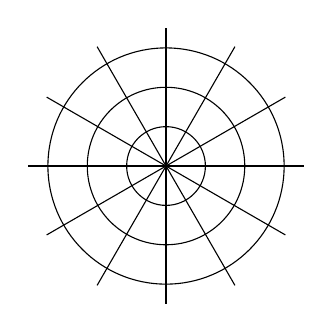
\begin{tikzpicture}[scale=0.5]
\foreach \r in {1, 2, 3} \draw (0,0) circle (\r);
\foreach \phi in {0, 30, ..., 360} \draw (0, 0) -- (\phi:3.5);
\end{tikzpicture}}
Нарисуйте, куда отображение $z\longmapsto z^2$ переводит\\
\пункт
декартову координатную сетку;\\
\пункт
полярную координатную сетку (см. рис.);\\
\пункт
окружность $|z+i|=1$;\\
\пункт
кошку (см. рис.)?\\
% \пункт
% Те же вопросы для отображения
% $z\longmapsto 1/z$.\\
\пункт[Инверсия]
пункты а--в для отображения $z\longmapsto 1/\bar z$.
\кзадача
\ВосстановитьГраницы





\пзадача
Докажите с помощью комплексных чисел, что
\невСтрочку
\пункт
композиция двух поворотов является поворотом или параллельным переносом;
\пункт
композиция поворота на ненулевой угол и параллельного переноса является поворотом.
\кзадача



%\задача
%Куда отображение $z\longmapsto\sqrt z$ переводит
%$\{z\in\Cbb\ |\ {\rm Im}\,(z)>0\}$?
%верхнюю полуплоскость (без границы)?
%\кзадача

% \задача
% Куда отображение\\
% \пункт
% $z\longmapsto1/z$;\\
% \спункт $z\longmapsto0,5(z+1/z)$\\
% переводит множество
% $\{z\in\Cbb\ |\ {\rm Im}\,(z)>0,\ |z|\leq1\}$?
%полукруг радиуса 1 с центром в начале координат, лежащий в верхней
%полуплоскости?
% \кзадача


%\сзадача
%Куда отображение  $z\longmapsto e^{z}$ переводит полосу
%$\{z\in\Cbb\ |\ 0\leq  {\rm Im}\,(z)< 2\pi\}$?
%полукруг радиуса 1 с центром в начале координат, лежащий в верхней
%полуплоскости?
%\кзадача

\vspace*{-1mm}


\ЛичныйКондуит{0mm}{5mm}

%\СделатьКондуит{3.7mm}{7.5mm}

% \GenXMLW
\end{document}





\задача
\вСтрочку
\пункт
Куда отображение $z\longmapsto1/z$ переводит
полукруг радиуса 1 с центром в начале координат, лежащий в верхней
полуплоскости?
\спункт Тот же вопрос для отображения
$z\longmapsto0,5(z+1/z)$.
\кзадача

\ЛичныйКондуит{0mm}{6mm}



%\СделатьКондуит{5mm}{7.5mm}





\end{document}

%\задача
%Нарисуйте образы следующих множеств при отображениях, задаваемых
%функциями:
%\вСтрочку
%\пункт $f(z)=\bar z$;\hfil
%\пункт $f(z)=z^n,\ n\in\N$;\\ \\ \\ \\ \\
%\пункт $f(z)=\sqrt z$;\hfil
%\пункт $f(z)=1/z$;\\ \\ \\ \\ \\
%\пункт $f(z)=e^z$;\hfil
%\пункт $f(z)=\sin z$;\\ \\ \\ \\ \\
%\пункт $f(z)=\cos z$;\hfil
%\спункт $f(z)=\tg z$;\\ \\ \\ \\ \\
%\спункт $f(z)=0,5(z+1/z)$.
%\кзадача




На прямоугольную карту положили карту той же
местности, но меньшего масштаба
(меньшая карта целиком лежит внутри большей).
Пусть масштаб первой карты в $k$ раз больше масштаба второй карты,
вторая карта сдвинута на вектор $z$ и повернута на угол $\alpha$
относительно первой карты. Найдите координаты точки, которая
изображает на обеих картах одну и ту же точку местности.

\задача
Докажите, что вещественная и мнимая части любого корня квадратного
уравнения с комплексными коэффициентами выражаются через вещественные
и мнимые части коэффициентов уравнения с помощью арифметических операций
и извлечения действительного
квадратного корня (т.~е.~\лк выражаются в радикалах\пк).
\кзадача

\задача
%\вСтрочку
%\пункт
Выразите в радикалах
$\cos\frac{2\pi}{5}$ и
$\sin\frac{4\pi}{5}$ и
%\кзадача
%\задача
%\пункт
постройте %при помощи
циркулем и линейкой правильный пятиугольник.
\кзадача 